\documentclass[conference]{IEEEtran}

% -------------------- Paketler --------------------
\usepackage[utf8]{inputenc}
\usepackage[T1]{fontenc}
\usepackage[turkish]{babel}
\usepackage{graphicx}
\usepackage{float}
\usepackage{booktabs}
\usepackage{array}
\usepackage{url}
\usepackage{hyperref}
\usepackage{amsmath}

\hypersetup{
    colorlinks=true,
    linkcolor=black,
    citecolor=black,
    urlcolor=blue
}

% -------------------- Başlık --------------------
\title{Büyük Ölçekli Sırt Çantası Problemlerinde Dinamik Programlama ve Genetik Algoritmanın Performans Analizi}

\author{
\IEEEauthorblockN{Halil Oğuz Çetin\IEEEauthorrefmark{1}, Edasu Kaya\IEEEauthorrefmark{2}}
\IEEEauthorblockA{
Manisa Celal Bayar Üniversitesi, Yazılım Mühendisliği Bölümü\\
\IEEEauthorrefmark{1}232803054 \quad
\IEEEauthorrefmark{2}232803046\\
\textbf{GitHub:} \href{https://github.com/HalilOguzCetin/knapsack-algorithm-analysis}{github.com/HalilOguzCetin/knapsack-algorithm-analysis}
}
}

\begin{document}

\maketitle

% -------------------- Özet --------------------
\begin{abstract}
Sırt Çantası Problemi (Knapsack Problem), sınırlı kapasiteye sahip bir çantaya en yüksek toplam değeri sağlayacak nesnelerin seçilmesini amaçlayan klasik bir kombinatoryal optimizasyon problemidir. Bu problem NP-Hard sınıfında yer aldığı için veri boyutu arttıkça kesin çözüm yöntemlerinin zaman ve bellek maliyeti artmaktadır. Bu çalışmada, Knapsack problemi üzerinde kesin çözüm yaklaşımı olan Dinamik Programlama (Dynamic Programming - DP) ile sezgisel çözüm yaklaşımı olan Genetik Algoritma (Genetic Algorithm - GA) karşılaştırılmıştır. Deneylerde farklı veri boyutları için algoritmaların çalışma süreleri, elde ettikleri çözüm değerleri ve optimum çözüme göre sapma oranları analiz edilmiştir. Sonuçlar, DP yönteminin optimum çözüme ulaşmada daha güvenilir olduğunu; GA yönteminin ise özellikle büyük ölçekli problemlerde daha hızlı ve kabul edilebilir çözümler üretebildiğini göstermektedir.
\end{abstract}

\begin{IEEEkeywords}
Knapsack Problemi, Dinamik Programlama, Genetik Algoritma, NP-Hard, Optimizasyon, Performans Analizi
\end{IEEEkeywords}

% -------------------- Giriş --------------------
\section{Giriş}
Optimizasyon problemleri, bilgisayar bilimlerinde ve mühendislik uygulamalarında sık karşılaşılan önemli problem türlerinden biridir. Bu problemlerde amaç, belirli kısıtlar altında en iyi çözümü elde etmektir. Sırt Çantası Problemi, bu alandaki en bilinen örneklerden biridir. Problemde her nesnenin bir ağırlığı ve değeri vardır. Amaç, çantanın kapasitesini aşmadan toplam değeri maksimum yapacak nesne kümesini seçmektir.

Knapsack problemi teorik olarak basit görünmesine rağmen, veri boyutu büyüdükçe çözüm uzayı hızlı şekilde genişler. Bu nedenle problem NP-Hard sınıfında değerlendirilir. Kesin çözüm yöntemleri optimum sonucu bulabilir; fakat büyük veri setlerinde zaman ve bellek kullanımı açısından maliyetli hale gelebilir. Sezgisel ve evrimsel algoritmalar ise optimum sonucu garanti etmese de daha kısa sürede kabul edilebilir sonuçlar üretebilir.

Bu çalışmanın amacı, Dinamik Programlama ve Genetik Algoritma yöntemlerini farklı veri boyutlarında karşılaştırarak doğruluk ve çalışma süresi açısından değerlendirmektir. Bu kapsamda N=50, N=200, N=1000, N=5000 ve N=10000 elemanlı veri setleri üzerinde deneyler gerçekleştirilmiştir.

% -------------------- Literatür --------------------
\section{Literatür Taraması}
Knapsack problemi, kombinatoryal optimizasyon literatüründe önemli bir yere sahiptir. Problem; kaynak tahsisi, bütçe planlama, proje seçimi, üretim planlama ve lojistik gibi birçok gerçek hayat problemine model oluşturabilmektedir.

Dinamik Programlama, Knapsack problemi için yaygın kullanılan kesin çözüm yöntemlerinden biridir. Bu yaklaşımda problem daha küçük alt problemlere ayrılır ve önceki hesaplamalar tekrar kullanılacak şekilde saklanır. Böylece aynı alt problemin tekrar tekrar çözülmesi engellenir. Ancak DP yönteminin zaman ve bellek karmaşıklığı, nesne sayısı ve kapasite değerine bağlı olarak artar.

Genetik Algoritma ise doğal seçilim ve evrimsel süreçlerden esinlenen sezgisel bir optimizasyon yöntemidir. Popülasyon, birey, uygunluk fonksiyonu, çaprazlama ve mutasyon gibi kavramlarla çalışır. GA, büyük arama uzaylarında hızlı şekilde iyi çözümler bulabilir. Ancak bulunan çözümün her zaman optimum olduğu garanti edilemez.

Bu nedenle literatürde Knapsack gibi NP-Hard problemlerde kesin algoritmalar ile sezgisel algoritmaların karşılaştırılması sıkça yapılmaktadır. Bu çalışma da aynı doğrultuda DP ve GA yöntemlerini deneysel olarak karşılaştırmaktadır.

% -------------------- Problem Tanımı --------------------
\section{Problem Tanımı}
Bu çalışmada ele alınan problem 0/1 Knapsack problemidir. Her nesne ya tamamen seçilir ya da hiç seçilmez. Parçalı seçim yapılmaz. Problem matematiksel olarak aşağıdaki şekilde ifade edilebilir:

\begin{equation}
\max \sum_{i=1}^{n} v_i x_i
\end{equation}

\begin{equation}
\sum_{i=1}^{n} w_i x_i \leq W
\end{equation}

\begin{equation}
x_i \in \{0,1\}
\end{equation}

Burada $v_i$ nesnenin değerini, $w_i$ nesnenin ağırlığını, $W$ çanta kapasitesini ve $x_i$ ilgili nesnenin seçilip seçilmediğini ifade etmektedir.

% -------------------- Yöntem --------------------
\section{Yöntem}
Bu çalışmada iki farklı algoritma kullanılmıştır: Dinamik Programlama ve Genetik Algoritma.

\subsection{Dinamik Programlama}
Dinamik Programlama yöntemi, problemi alt problemlere bölerek çözen kesin bir yaklaşımdır. Bu yöntemde her nesne ve kapasite durumu için en iyi değer hesaplanır. DP tablosunda tutulan değerler sayesinde önceki sonuçlar tekrar kullanılır.

DP yönteminin en önemli avantajı optimum sonucu garanti etmesidir. Ancak kapasite ve nesne sayısı büyüdükçe tablo boyutu da büyür. Bu durum özellikle büyük veri setlerinde zaman ve bellek maliyetini artırır.

\subsection{Genetik Algoritma}
Genetik Algoritma, başlangıçta rastgele oluşturulan bireylerden meydana gelen bir popülasyon ile çalışır. Her birey, problem için olası bir çözümü temsil eder. Knapsack probleminde bireyler, nesnelerin seçilip seçilmediğini gösteren ikili diziler şeklinde modellenebilir.

Algoritmada her bireyin uygunluk değeri hesaplanır. Kapasite sınırını aşmayan ve daha yüksek toplam değer sağlayan bireyler daha başarılı kabul edilir. Daha sonra seçim, çaprazlama ve mutasyon işlemleriyle yeni nesiller oluşturulur. Bu süreç belirli bir iterasyon sayısına kadar devam eder.

GA yönteminin avantajı büyük çözüm uzaylarında hızlı şekilde iyi sonuçlar üretebilmesidir. Dezavantajı ise optimum sonucu garanti etmemesidir.

% -------------------- Deneysel Kurulum --------------------
\section{Deneysel Kurulum}
Deneylerde farklı büyüklüklerde veri setleri kullanılmıştır. Her veri setinde nesneler ağırlık ve değer bilgileriyle temsil edilmiştir. Algoritmalar aynı veri setleri üzerinde çalıştırılmış ve sonuçlar karşılaştırılmıştır.

Karşılaştırmada üç temel ölçüt kullanılmıştır:

\begin{itemize}
    \item \textbf{Çalışma Süresi:} Algoritmanın sonucu üretmek için harcadığı süre.
    \item \textbf{Çözüm Değeri:} Algoritmanın elde ettiği toplam değer.
    \item \textbf{Sapma Oranı:} GA sonucunun DP sonucuna göre ne kadar uzak olduğunu gösteren oran.
\end{itemize}

Sapma oranı aşağıdaki formül ile hesaplanmıştır:

\begin{equation}
Sapma(\%) = \frac{DP\ Degeri - GA\ Degeri}{DP\ Degeri} \times 100
\end{equation}

% -------------------- Sonuçlar --------------------
\section{Deneysel Sonuçlar ve Analiz}
Algoritmaların farklı veri boyutlarındaki sonuçları Tablo~\ref{tab:results} üzerinde gösterilmiştir.

\begin{table}[H]
\centering
\caption{DP ve GA Algoritmalarının Karşılaştırılması}
\label{tab:results}
\resizebox{\columnwidth}{!}{%
\begin{tabular}{cccccc}
\toprule
\textbf{N} & \textbf{DP Değer} & \textbf{GA Değer} & \textbf{Sapma (\%)} & \textbf{DP Süre (s)} & \textbf{GA Süre (s)} \\
\midrule
50    & 2425  & 2251.0  & 7.17  & 0.00902 & 0.01150 \\
200   & 5597  & 916.5   & 83.63 & 0.03930 & 0.03767 \\
1000  & 12216 & 3679.0  & 69.89 & 0.19527 & 0.17997 \\
5000  & 24426 & 16031.6 & 34.38 & 1.03483 & 0.95387 \\
10000 & 32775 & 30837.6 & 5.91  & 2.00310 & 1.84998 \\
\bottomrule
\end{tabular}%
}
\end{table}

% -------------------- Grafikler --------------------

\clearpage
\onecolumn

\begin{figure}[H]
\centering

\includegraphics[width=0.82\textwidth]{runtime_graph.png}
\caption{Algoritmaların çalışma süresi karşılaştırması}
\label{fig:runtime}
\end{figure}

\vspace{0.4cm}

\begin{figure}[H]
\centering
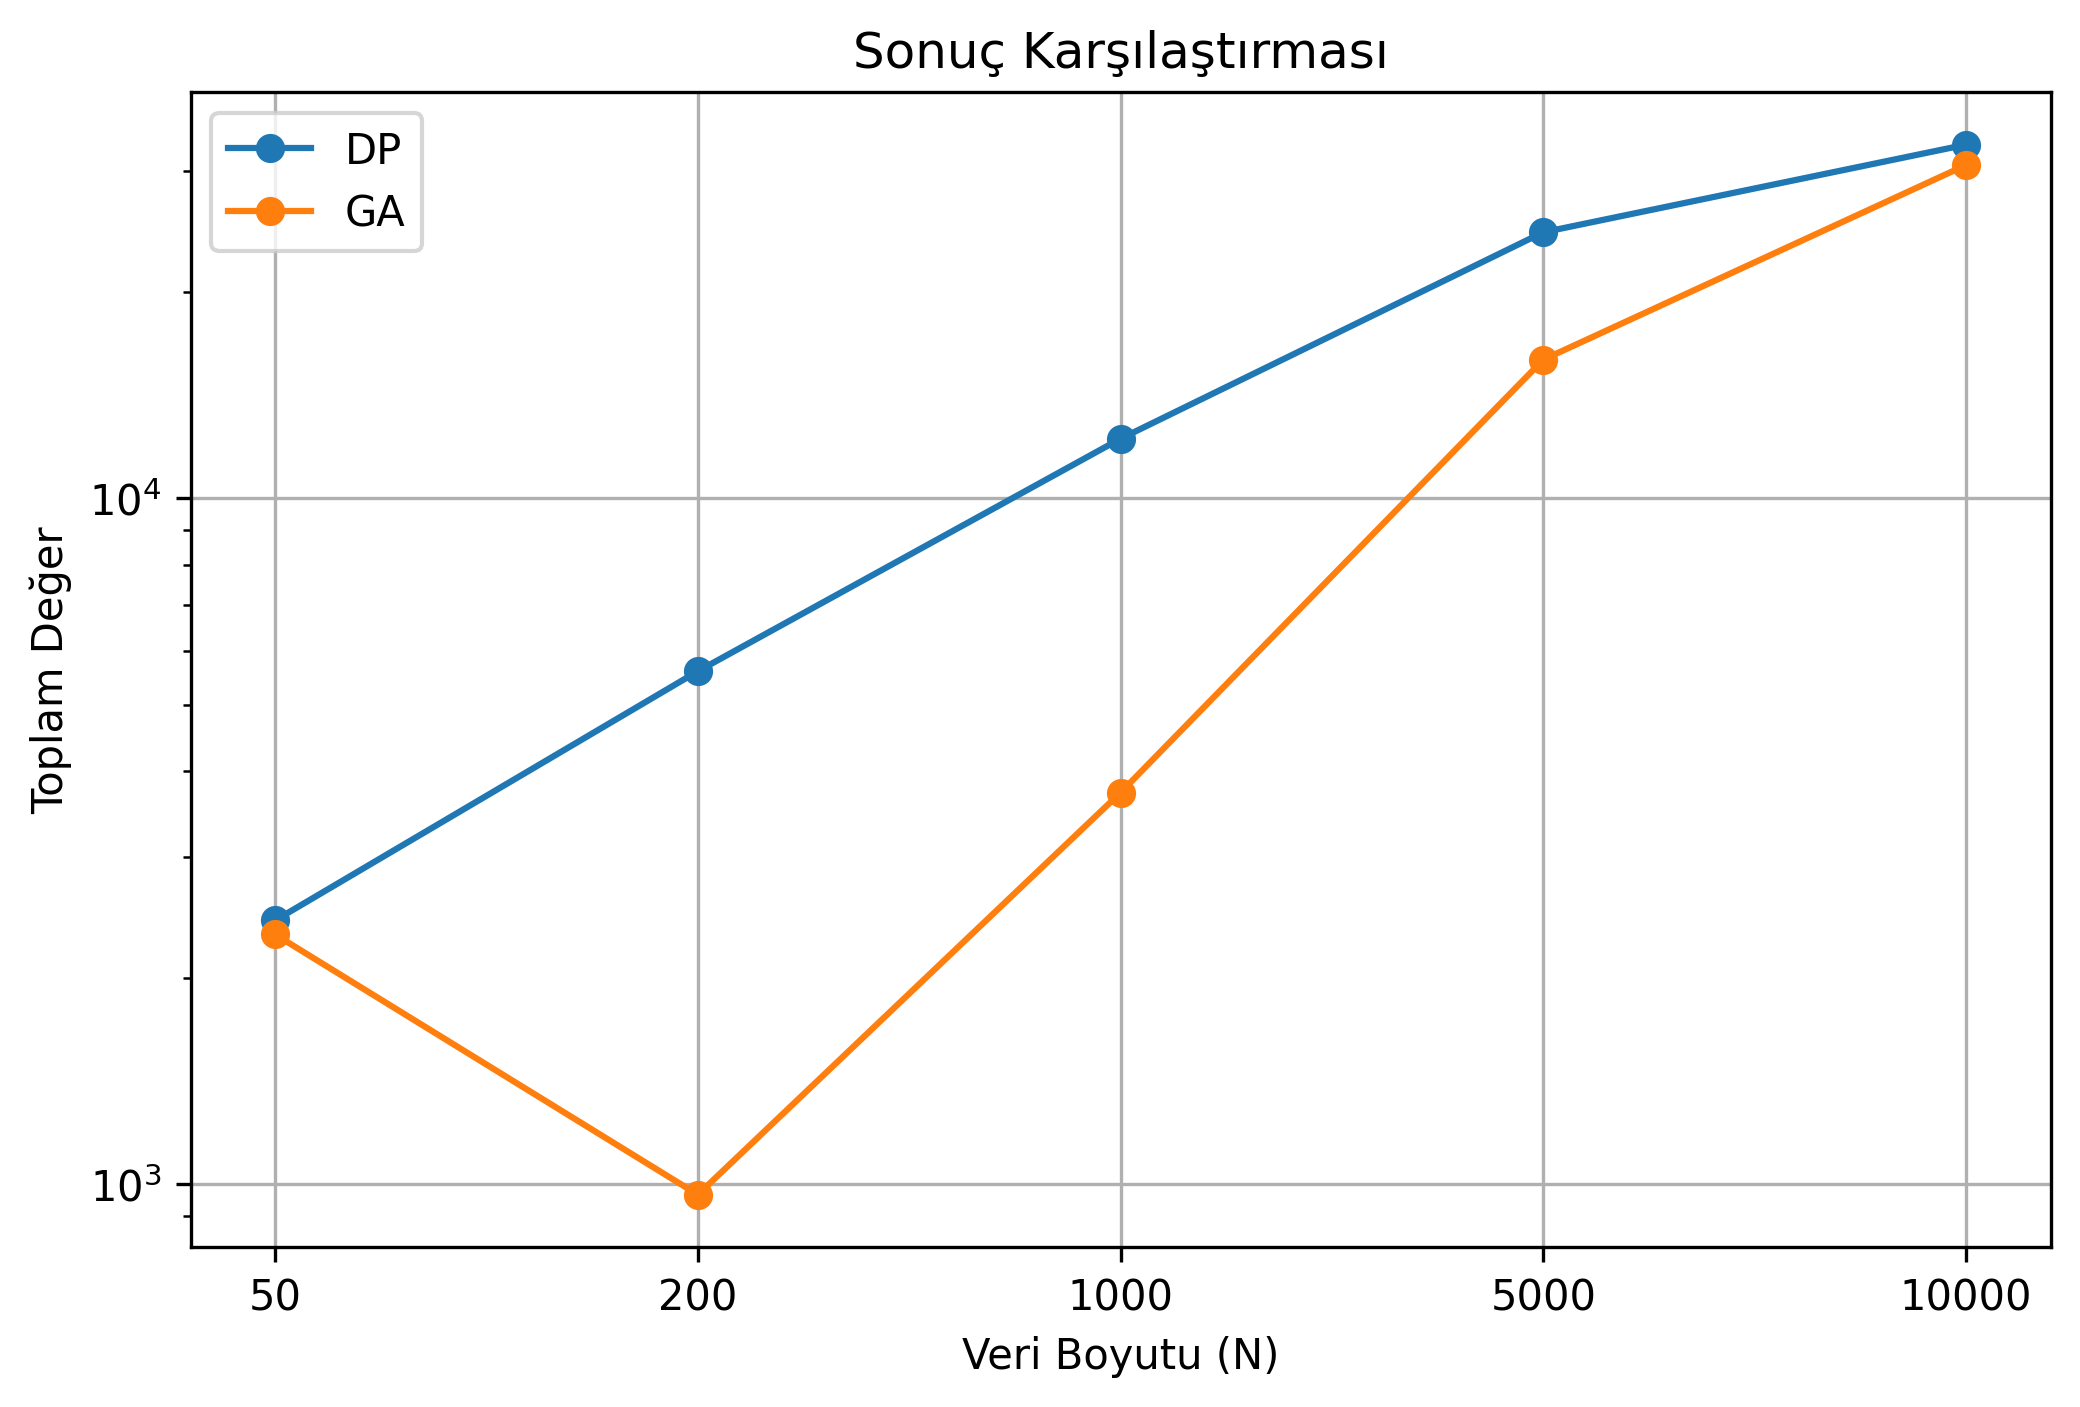
\includegraphics[width=0.82\textwidth]{accuracy_graph.png}
\caption{Algoritmaların çözüm değeri karşılaştırması}
\label{fig:accuracy}
\end{figure}

\vspace{0.4cm}

\begin{figure}[H]
\centering
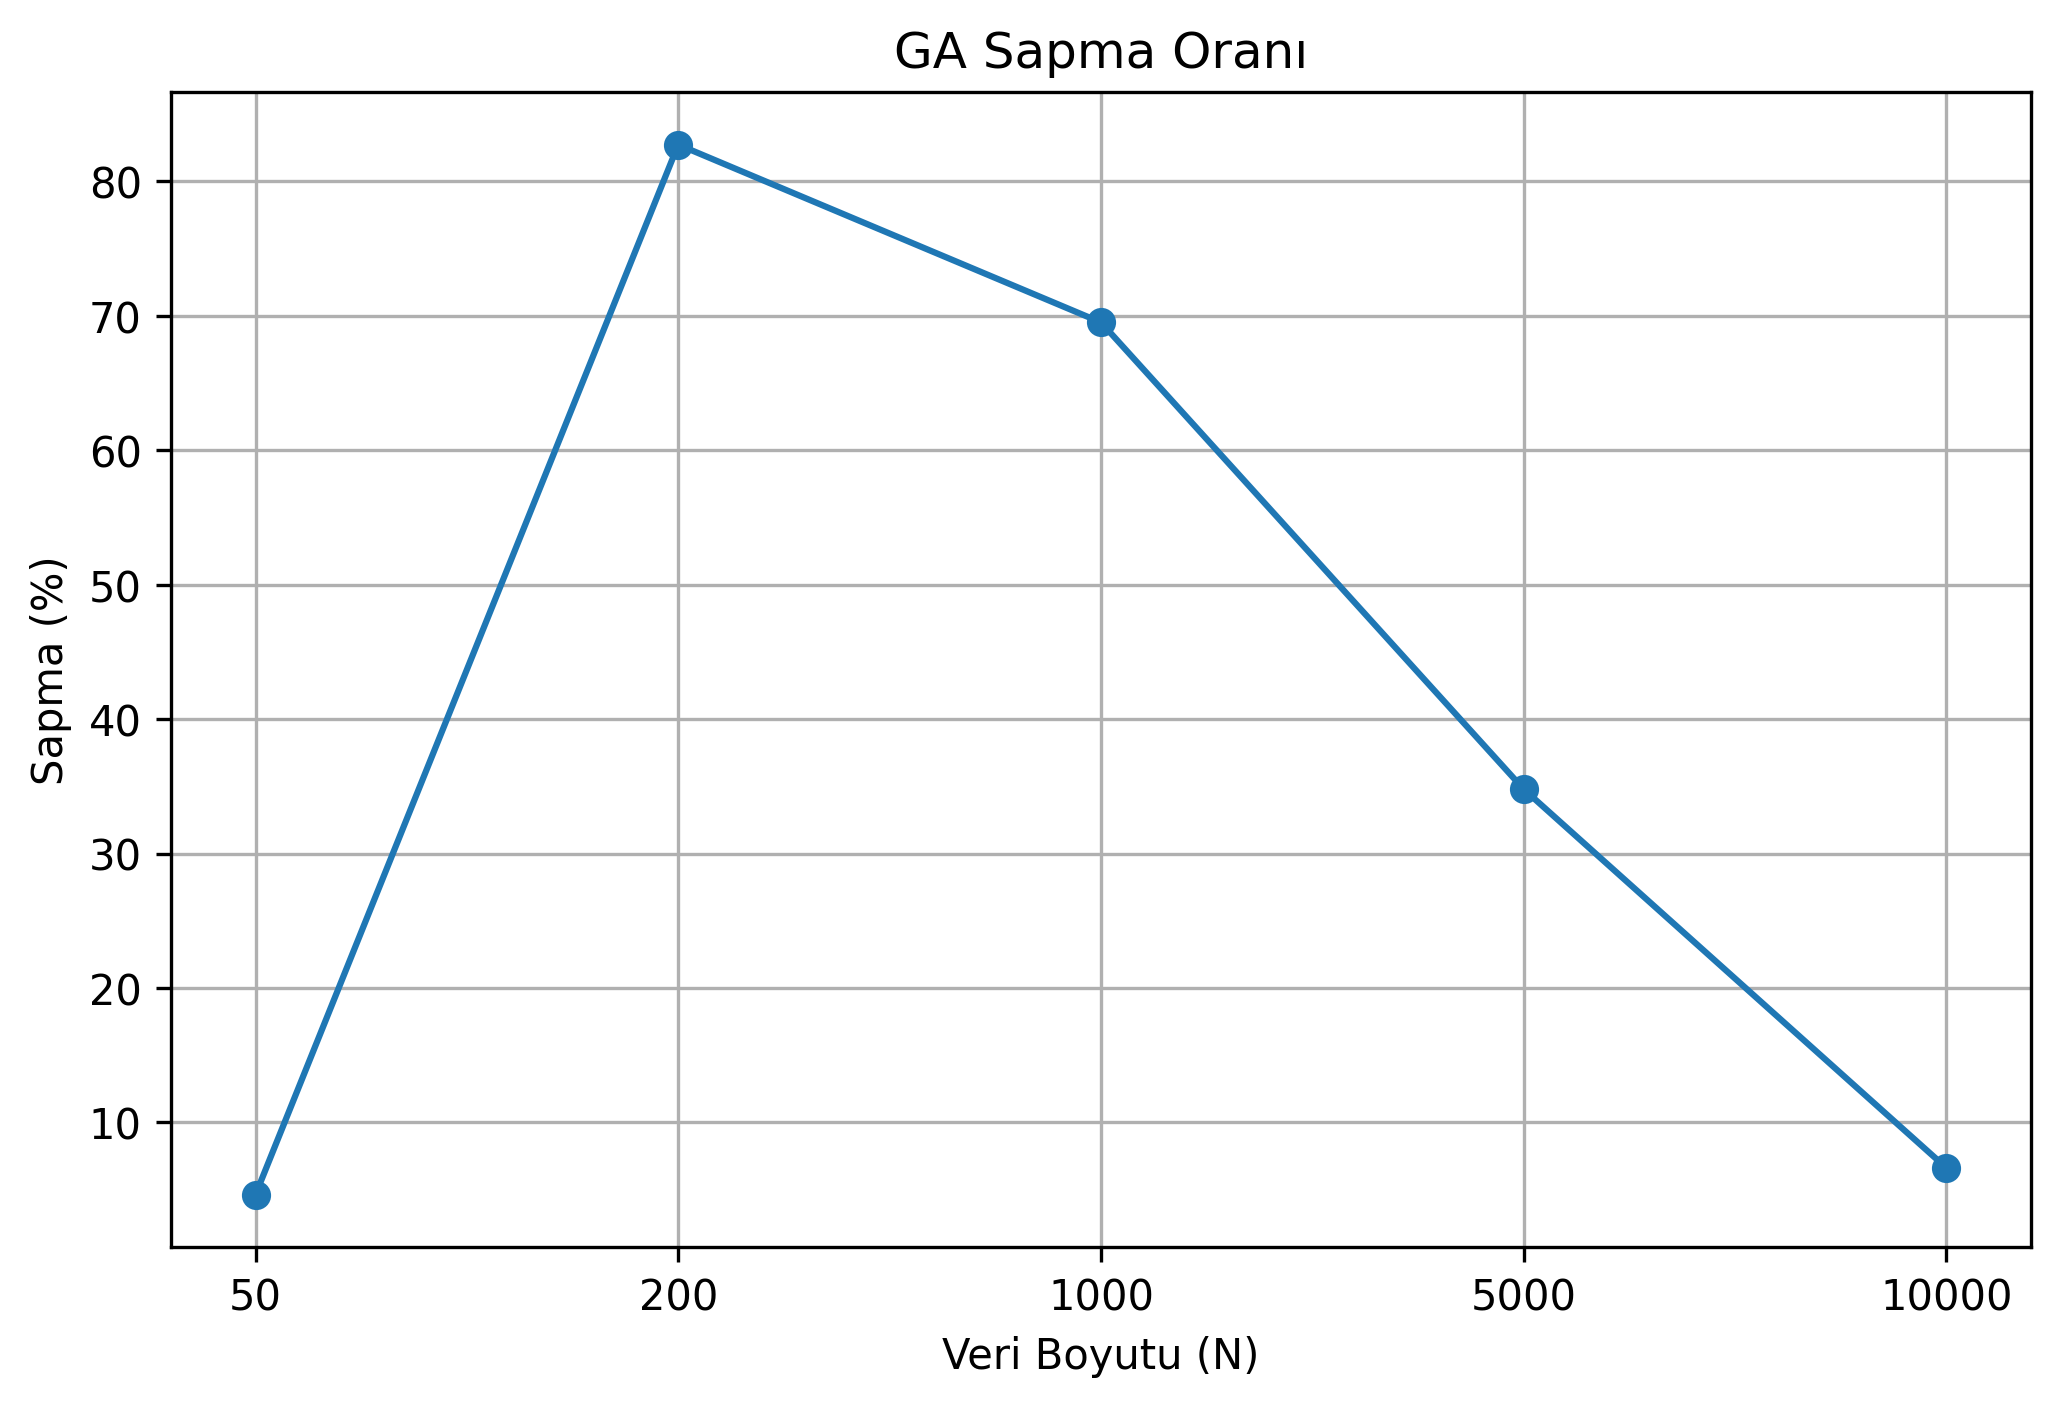
\includegraphics[width=0.82\textwidth]{gap_graph.png}
\caption{Genetik Algoritmanın DP sonucuna göre sapma oranı}
\label{fig:gap}
\end{figure}

\clearpage
\twocolumn

Tablo~\ref{tab:results} incelendiğinde, Dinamik Programlama algoritmasının tüm veri boyutlarında Genetik Algoritmaya göre daha yüksek çözüm değeri ürettiği görülmektedir. Bu beklenen bir durumdur; çünkü DP yöntemi kesin çözüm yaklaşımıdır ve optimum sonucu hedefler.

Çalışma süreleri incelendiğinde, veri boyutu arttıkça her iki algoritmanın da çalışma süresi artmaktadır. Deneylerde N=50 ve N=200 için iki algoritmanın süreleri birbirine çok yakınken, veri boyutu büyüdükçe süre farkı daha belirgin hale gelmiştir. N=10000 veri setinde DP 2.00310 saniyede, GA ise 1.84998 saniyede çalışmıştır. Bu sonuç, GA yönteminin büyük veri setlerinde süre açısından avantaj sağlayabileceğini göstermektedir.

GA sonuçlarında sapma oranı veri setlerine göre değişiklik göstermektedir. Özellikle N=200 ve N=1000 için GA'nın optimumdan belirgin şekilde uzaklaştığı görülmektedir. Buna karşılık N=10000 veri setinde sapma oranı \%5.91 seviyesine düşmüştür. Bu sonuç, GA'nın bazı büyük veri setlerinde optimuma yakın ve daha hızlı sonuçlar üretebildiğini göstermektedir.

Genel olarak DP doğruluk açısından daha başarılıdır. GA ise optimum garantisi vermemesine rağmen hız ve ölçeklenebilirlik açısından avantaj sağlayabilecek bir yöntemdir. Bu durum, kesin algoritmalar ile sezgisel algoritmalar arasındaki temel dengeyi göstermektedir.

% -------------------- Tartışma --------------------
\section{Tartışma}
Elde edilen sonuçlar, algoritma seçiminin problemin büyüklüğüne ve beklenen doğruluk seviyesine göre yapılması gerektiğini göstermektedir. Küçük ve orta ölçekli problemlerde optimum sonuç gerekli ise DP yöntemi tercih edilebilir. Ancak veri boyutu çok büyüdüğünde veya kısa sürede yaklaşık bir sonuç yeterli olduğunda GA gibi sezgisel yöntemler daha kullanışlı olabilir.

Bu çalışmada DP algoritması N=10000 değerine kadar çalıştırılmıştır. Ancak DP'nin gerçek sınırı yalnızca nesne sayısına değil, aynı zamanda kapasite değerine de bağlıdır. Kapasite değeri büyüdükçe DP tablosu büyüyeceği için bellek tüketimi artacaktır. Bu nedenle daha yüksek kapasite değerlerinde DP'nin performansı daha hızlı düşebilir.

GA'nın başarısı ise popülasyon büyüklüğü, nesil sayısı, çaprazlama oranı ve mutasyon oranı gibi parametrelere bağlıdır. Bu parametreler iyileştirildiğinde GA'nın optimuma daha yakın sonuçlar üretmesi mümkündür.

% -------------------- Sonuç --------------------
\section{Sonuç}
Bu çalışmada 0/1 Knapsack problemi üzerinde Dinamik Programlama ve Genetik Algoritma yöntemleri karşılaştırılmıştır. Deneysel sonuçlara göre DP algoritması tüm veri setlerinde daha yüksek çözüm değeri üretmiş ve doğruluk açısından daha başarılı olmuştur. Bunun temel nedeni DP'nin kesin çözüm yaklaşımı olmasıdır.

Genetik Algoritma ise optimum sonucu garanti etmemesine rağmen bazı büyük veri setlerinde optimuma yakın sonuçlar üretebilmiştir. Özellikle N=10000 veri setinde GA'nın sapma oranının \%5.91 olması, sezgisel yöntemlerin büyük ölçekli problemlerde kabul edilebilir sonuçlar sağlayabileceğini göstermektedir.

Bu çalışmada DP algoritması N=10000 değerine kadar çalışmıştır; ancak veri boyutu ve kapasite arttıkça zaman ve bellek maliyeti nedeniyle daha büyük problemlerde uygulanabilirliği azalabilir. GA ise daha esnek bir yöntem olarak büyük veri setlerinde alternatif bir çözüm yaklaşımı sunmaktadır.

Gelecek çalışmalarda Genetik Algoritma parametreleri optimize edilerek daha düşük sapma oranları elde edilebilir. Ayrıca Simulated Annealing, Greedy algoritmalar ve hibrit yöntemler de karşılaştırmaya dahil edilerek daha kapsamlı bir analiz yapılabilir.

% -------------------- Kaynakça --------------------
\begin{thebibliography}{9}

\bibitem{cormen}
T. H. Cormen, C. E. Leiserson, R. L. Rivest, and C. Stein, \textit{Introduction to Algorithms}. MIT Press, 2009.

\bibitem{goldberg}
D. E. Goldberg, \textit{Genetic Algorithms in Search, Optimization and Machine Learning}. Addison-Wesley, 1989.

\bibitem{martello}
S. Martello and P. Toth, \textit{Knapsack Problems: Algorithms and Computer Implementations}. Wiley, 1990.

\bibitem{garey}
M. R. Garey and D. S. Johnson, \textit{Computers and Intractability: A Guide to the Theory of NP-Completeness}. W. H. Freeman, 1979.

\end{thebibliography}

\end{document}